\section{Pipeline Documentaire}\label{sec:pipeline-documentaire}

Cette première section plonge au cœur du projet Pipeline documentaire. Je commencerai par examiner le processus d'installation du projet dans un environnement de développement. Cela inclura la préparation de l'infrastructure nécessaire (conteneurs Docker) à l'exécution de l'API et la configuration de Laravel. De plus, je me pencherai sur les migrations de base de données indispensables pour assurer la cohérence des données et le bon fonctionnement de l'API. La section se poursuivra en explorant les modèles qui correspondent aux tables de la base de données.

Le cœur de cette section portera sur le processus clé de l'API : l'importation d'un fichier. Je décomposerai ce processus complexe en étapes gérables, en mettant en évidence les opérations importantes qui se produisent en arrière-plan lorsqu'un fichier est soumis à l'API. Des exemples de code accompagneront cette exploration, illustrant chaque étape du processus.

Enfin, j'aborderai l'aspect crucial des tests. La fiabilité et la robustesse de l'API sont essentielles pour assurer un fonctionnement sans faille.

En somme, cette première section plongera profondément dans l'API Pipeline documentaire, de sa mise en place à son fonctionnement concret. Chaque aspect exploré contribuera à la construction d'une base solide pour la section suivante, où j'examinerai l'intégration de l'API dans une mission frontend spécifique.

\subsection{Installation pour le développement}

Pour amorcer le développement de l'API, il est impératif de cloner deux projets à partir du dépôt GitLab de l'entreprise. Le premier de ces projets, intitulé \Verb|pipelinedoc-docker|, renferme un ensemble de fichiers essentiels. Ce dépôt inclut notamment un \Verb|Dockerfile| (\Verb|app.dockerfile|) ainsi qu'un fichier \Verb|docker-compose.yml|. Il abrite également une structure de dossiers (Figure~\ref{fig:pipelinedoc-docker-folders}) comprenant le fichier de configuration Nginx (\Verb|app.conf|), le répertoire destiné au code de l'API (\Verb|apps|) ainsi que d'autres dossiers de substitution nécessaires au projet.

\begin{wrapfigure}{l}{0.32\textwidth}
    \centering
    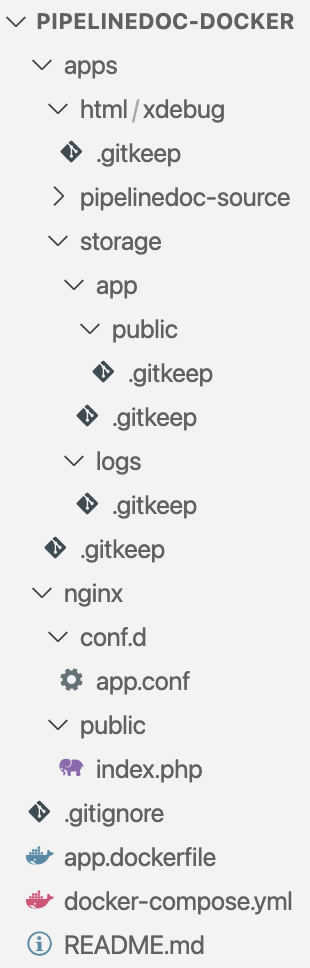
\includegraphics[width=0.30\textwidth]{img/pipelinedoc-docker-folders}
    \caption{La structure des dossiers du projet \Verb{pipelinedoc-docker}.}
    \label{fig:pipelinedoc-docker-folders}
\end{wrapfigure}

Le second projet, baptisé \Verb|pipelinedoc-source|, renferme le code source de l'API Pipeline documentaire. Ce dernier devra être cloné dans le dossier approprié au sein du projet \Verb|pipelinedoc-docker|. Cette étape est primordiale pour établir la connexion entre l'infrastructure Docker mise en place et le code de l'API à développer.

Les fichiers \Verb|app.dockerfile|, \Verb|docker-compose.yml| et le fichier de configuration Nginx sont essentiellement les mêmes que les fichiers présentés pour la production (Code source~\ref{code:dockerfile-prod}, page~\pageref{code:dockerfile-prod}; Code source~\ref{code:docker-compose-prod}, page~\pageref{code:docker-compose-prod}; Code source~\ref{code:nginx-conf-prod}, page~\pageref{code:nginx-conf-prod}). Cependant, bien qu'ils soient plus simples, ils ne contiennent pas toutes les instructions présentes dans ces fichiers.

Dès que les deux projets sont clonés, les conteneurs Docker peuvent être démarrés avec la commande suivante : \Verb|docker compose up|. Ensuite, le développeur doit créer le fichier \Verb|.env| pour le projet, contenant toutes les variables environnementales nécessaires, telles que les détails des connexions à la base de données, les URL et les jetons vers d'autres services, ainsi que d'autres paramètres de configuration. L'étape suivante consiste à installer les dépendances avec la commande \Verb|composer install| et à les mettre à jour avec la commande \Verb|composer update|. Ces commandes utilisent le fichier \Verb|composer.json| pour installer et mettre à jour les dépendances répertoriées avec leurs numéros de version. Ce projet inclut non seulement des dépendances publiques, mais également des dépendances développées et maintenues par l'entreprise dans son propre dépôt privé. Ces paquets privés sont ce que l'on appelle les \foreignquote{french}{cores}, comme nous l'avons mentionné précédemment (Figure~\ref{fig:architecture}, page~\pageref{fig:architecture}; Sous-section~\ref{subsec:cores}, page~\pageref{subsec:cores}).

Il reste encore trois petites étapes pour installer et démarrer complètement le projet : il faut lancer la commande \Verb|php artisan migrate:install|\footnote{Artisan est l'outil de ligne de commande intégré de Laravel, permettant d'effectuer diverses tâches liées au développement et à la gestion de projets Laravel.} pour créer la table \Verb|migrations| dans la base de données. Ensuite, il faut exécuter la commande \Verb|php artisan migrate| pour créer les tables nécessaires au projet, qui sont définies dans les fichiers de migration situés dans le dossier \Verb|database/migrations| du projet Laravel. Enfin, il faut utiliser la commande \Verb|php artisan queue:listen|\footnote{Ces commandes doivent bien sûr être exécutées dans le conteneur de l'application et à partir de son dossier racine.} pour démarrer la file d'attente de Laravel. À ce stade, le système est prêt à importer des fichiers et à exécuter ses autres fonctionnalités. Dans les lignes qui suivent, j'examinerai un peu plus en détail les fichiers de migration qui définissent la structure des tables de la base de données nécessaires au projet.
\subsection{Migrations de la base de données}

Les migrations dans Laravel sont un mécanisme permettant de gérer et de maintenir la structure de la base de données d'une application de manière efficace et contrôlée. Les migrations définissent les schémas des tables de la base de données, ainsi que les modifications ultérieures à ces schémas. Elles offrent un moyen de collaborer entre développeurs en suivant un processus de versionnement pour les modifications de la base de données.

Pour créer une migration, on utilise l'outil de ligne de commande Artisan fourni par Laravel, en exécutant la commande \Verb|php artisan make:migration|. Cette commande génère un fichier de migration dans le répertoire \Verb|database/migrations| du projet. Dans ce fichier, on peut définir les colonnes de la table, les clés étrangères, les index, etc.

Une fois la migration créée, on peut exécuter la commande \Verb|php artisan migrate| pour appliquer les migrations en attente et mettre à jour la base de données selon les schémas définis. Les migrations permettent également de revenir en arrière en cas de besoin avec la commande \Verb|php artisan migrate:rollback|.

L'utilisation des migrations permet aux développeurs de travailler de manière collaborative et organisée en maintenant un historique des changements de structure de la base de données. Cela facilite également le déploiement sur différents environnements et assure une gestion centralisée de la structure de la base de données au sein du code source du projet.

Comme le modèle physique de données (Figure~\ref{fig:pmd}, page~\pageref{fig:pmd}) l'a défini, nous avons créé trois tables dans la base de données à l'aide de fichiers de migration : la table des téléchargements (\Verb|uploads|), la table des étapes des téléchargements (\Verb|upload_step|) et la table des résultats des téléchargements \Verb|upload_results|. À titre d'exemple, le fichier de migration de la table \Verb|uploads| est présenté dans le Code source~\ref{code:uploads-migration}.

Cette migration crée une table nommée \Verb|uploads| avec plusieurs colonnes :

\begin{itemize}
    \item \textbf{\Verb|id|} : Une clé primaire unique générée à l'aide d'ULID (Universally Unique Lexicographically Sortable Identifier).
    \item \textbf{\Verb|parameters|} : Une colonne de type JSON pour stocker des paramètres au format JSON.
    \item \textbf{\Verb|client_app|} : Une colonne de type entier pour enregistrer l'application cliente.
    \item \textbf{\Verb|upload_type|} : Une colonne de type chaîne de caractères (string) pour spécifier le type de téléchargement.
    \item \textbf{\Verb|status|} : Une colonne de type entier avec une valeur par défaut de 0, représentant l'état du téléchargement (0 : reçu, 1 : démarré, 2 : en attente, 3 : terminé, 4 : abandonné).
    \item \textbf{\Verb|timestamps|} : Deux colonnes pour enregistrer les horodatages de création et de mise à jour des enregistrements.
    \item \textbf{\Verb|deleted_at|} : Une colonne pour prendre en charge la suppression douce (soft delete) avec une précision temporelle de 0.
\end{itemize}

\begin{code}
    \caption{La classe de migration de la table \Verb{uploads}.}
    \inputminted{php}{code/2022_12_20_111202_create_uploads_table.php}
    \label{code:uploads-migration}
\end{code}

La méthode \mintinline{php}|up()| est utilisée pour créer la table avec les colonnes spécifiées, tandis que la méthode \mintinline{php}|down()| est utilisée pour supprimer la table en cas de rollback. Le code est encapsulé dans une classe anonyme héritant de la classe de migration. Cela permet de créer et exécuter la migration sans avoir à nommer explicitement la classe de migration, ce qui est courant dans les fichiers de migration Laravel.

L'objet \mintinline{php}|$table|, au sein de la classe de migration, représente l'entité qui permet de définir et de structurer la table de base de données au moyen de la migration. Dans le contexte de Laravel, cet objet est une instance de la classe \mintinline{php}|Blueprint|, qui offre un ensemble de méthodes et de fonctionnalités pour concevoir la structure de la table de manière programmatique.

    Chaque méthode appelée sur l'objet \mintinline{php}|$table| correspond à une opération spécifique permettant de construire la table. Ceci facilite la création cohérente et reproductible de la base de données. Par exemple, dans ce cas, les instructions telles que \mintinline{php}|$table->ulid('id')->primary()| définissent la colonne \Verb|id| comme une clé primaire dotée d'une valeur unique générée par le biais d'ULID. De la même manière, d'autres méthodes comme \mintinline{php}|$table->json('parameters')|, \mintinline{php}|$table->integer('client_app')|, etc., définissent les colonnes de la table et leurs types de données respectifs.

    L'objet \mintinline{php}|$table| revêt une importance fondamentale au sein du processus de migration Laravel. Il agit comme un canal permettant de décrire, de manière systématique, la structure de la table de base de données. Ce mécanisme offre une approche structurée et organisée pour gérer les changements de schéma de la base de données de manière réversible et documentée.

La structure des fichiers de migration des deux autres tables est similaire à celle-ci, avec des colonnes différentes bien sûr. Ces deux tables sont dans une relation un-à-plusieurs avec la table \Verb|uploads|, donc elles ont des clés étrangères comme l'une de leurs colonnes créées par le code suivant dans leurs fichiers de migration : \mintinline{php}|$table->foreignUlid('upload_id')->constrained('uploads');|.

Laravel utilise les informations dans des fichiers des migrations pour générer automatiquement les requêtes SQL nécessaires. Cela se traduit par la création, la modification ou la suppression des tables et des colonnes dans la base de données sous-jacente. Par exemple, le code SQL généré par Laravel à partir du fichier de migration de la table \Verb{uploads} est présenté dans le Code source~\ref{code:uploads-sql}.

\begin{code}
    \caption{Le code SQL généré par Laravel sur la base du fichier de migration de la table \Verb{uploads}.}
    \inputminted{sql}{code/uploads.sql}
    \label{code:uploads-sql}
\end{code}
\subsection{Modèles}

Les modèles dans Laravel sont des représentations essentielles des tables de la base de données au sein de l'application. Ils agissent comme des intermédiaires entre les données stockées dans la base de données et la logique métier de l'application. Chaque modèle est associé à une table spécifique dans la base de données et permet d'effectuer des opérations courantes, telles que la création, la lecture, la mise à jour et la suppression (CRUD), sur les données de cette table. Les modèles fournissent également des mécanismes pour définir des relations entre les tables, comme les relations un-à-un, un-à-plusieurs et plusieurs-à-plusieurs. Grâce aux modèles, les développeurs peuvent interagir avec la base de données de manière conviviale et orientée objet, sans avoir à écrire directement des requêtes SQL complexes. En encapsulant la logique de manipulation des données, les modèles contribuent à la clarté, à la maintenabilité et à la robustesse du code de l'application Laravel.

Les modèles sont créés dans Laravel en utilisant l'outil de ligne de commande Artisan. Pour générer un modèle, on exécute la commande \Verb|php artisan make:model NomDuModele|. Cette commande génère automatiquement une classe modèle dans le répertoire \Verb|app/Models| du projet. Cette classe étend la classe de base \Verb|Illuminate\Database\Eloquent\Model|, ce qui permet au modèle d'hériter de fonctionnalités essentielles offertes par Eloquent, le moteur de requête ORM de Laravel. Une fois le modèle créé, on peut définir les propriétés, les relations avec d'autres modèles et les méthodes spécifiques nécessaires pour interagir avec la base de données et manipuler les données associées à la table correspondante.

Comme démontré dans la sous-section précédente, nous avons créé trois tables dans la base de données à l'aide des migrations. Par conséquent, nous avons ensuite mis en place trois modèles correspondant à ces tables : \Verb|Upload|, \Verb|UploadStep| et \Verb|UploadResult|. À titre d'exemple, le code source du modèle \Verb|Upload| sera détaillé ici (Code source~\ref{code:uploads-model}).

\begin{code}
    \caption{Une version simplifiée du modèle \Verb{Upload}.}
    \inputminted{php}{code/Upload.php}
    \label{code:uploads-model}
\end{code}

La classe \Verb|Upload| est située dans l'espace de noms \Verb|App\Models|. Elle utilise la fonctionnalité \Verb|HasUlids| pour gérer les ULIDs (Universally Unique Lexicographically Sortable Identifier) pour l'identifiant primaire de la table. Les propriétés \Verb|$fillable| définissent les champs de la table qui peuvent être mass-assignés et \Verb|$hidden| détermine les champs qui ne seront pas inclus lors de la conversion en tableau ou en JSON.

Le modèle utilise la fonction de casting \Verb|$casts| pour traiter le champ \Verb|parameters| comme un tableau JSON. De plus, il définit deux relations \Verb|HasMany| : \Verb|steps()| pour représenter une relation un-à-plusieurs avec le modèle \Verb|UploadStep| et \Verb|results()| pour une relation similaire avec le modèle \Verb|UploadResult|. Ces relations permettent d'accéder facilement aux étapes et aux résultats associés à un objet \Verb|Upload|.

En outre, le modèle possède une méthode \Verb|setStatus()| qui permet de définir l'état de téléchargement des documents. Cette méthode utilise la classe \Verb|UploadStatus| pour traduire le code d'état en une valeur compréhensible et met à jour la base de données avec la nouvelle valeur.

En somme, le modèle \Verb|Upload| facilite la manipulation des données de la table associée, en fournissant des méthodes pour gérer les relations et les opérations spécifiques, tout en maintenant une cohérence entre la logique de l'application et les données stockées.
\subsection{Le processus d'importation d'un fichier}

Dans cette sous-section, nous suivrons le destin d'un fichier pendant son importation, depuis son arrivée à l'API dans le corps d'une requête POST, jusqu'à l'enregistrement de ses données dans la table appropriée de la base de données adéquate. Nous utiliserons à titre d'exemple un fichier LCCC (La Compagnie des Cartes Carburant SAS) qui est un type de fichier de transactions de carburant au format \Verb|csv| (Figure~\ref{fig:lccc}).

\begin{figure}[ht]
    \centering
    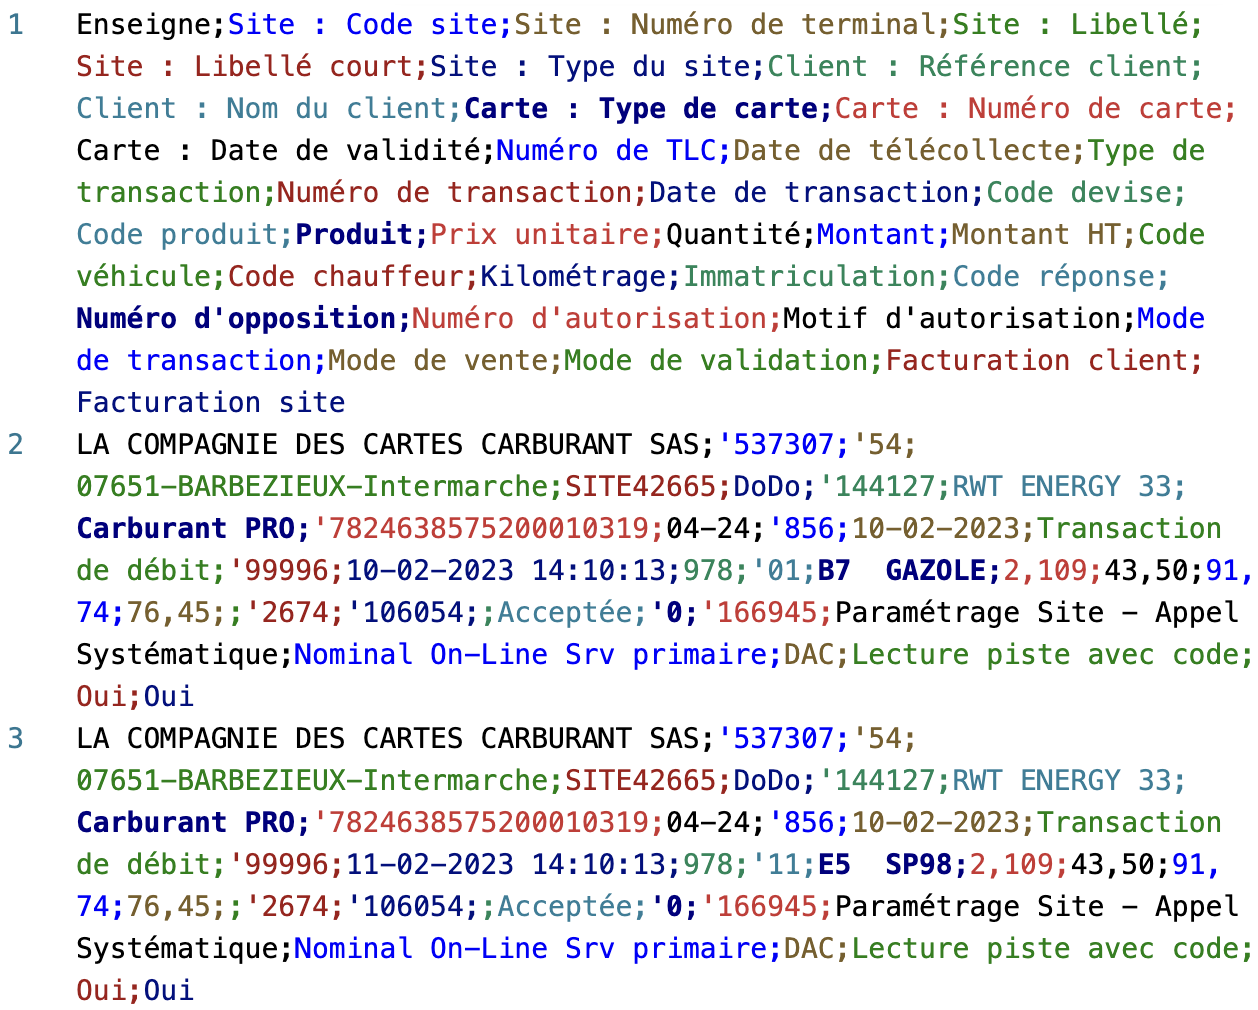
\includegraphics[width=\textwidth]{img/lccc-csv}
    \caption{Exemple d'un fichier LCCC.}
    \label{fig:lccc}
\end{figure}

Pour l'API, il est possible d'envoyer des fichiers dans le corps d'une requête POST au format encodé en base64, en tant que partie d'un objet JSON bien défini, comme démontré dans le Code source~\ref{code:lccc-payload}. Cette charge utile est validée avant d'être acceptée par l'API, plus précisément l'application Laravel utilise la méthode \Verb|rules()| de la classe \Verb|UploadStoreRequest| créée par nous pour la valider (Code source~\ref{code:upload-store-request}).

Cette classe se trouve dans le dossier \Verb|app/Http/Requests|. Elle étend la classe \Verb|FormRequest| de Laravel, permettant ainsi de définir les règles de validation pour la requête de stockage (store request) d'import de fichiers.

La méthode \Verb|rules()| définit les règles de validation pour les différentes parties de la requête. Les règles sont définies sous forme d'un tableau associatif. Parmi les règles définies :

\begin{itemize}
    \item Le champ \Verb|client_app| doit être présent, être un nombre entier et être une des valeurs autorisées spécifiées dans la configuration du projet (\Verb|allowed_client_app|).
    \item Le champ \Verb|parameters| doit être un tableau avec au moins deux éléments.
    \item Les éléments spécifiques du champ \Verb|parameters| (\Verb|client_id| et \Verb|user_id|) doivent être présents, être des nombres entiers et être obligatoires.
    \item Le champ \Verb|files| doit être un tableau avec au moins un élément.\footnote{Pour l'instant, l'API n'est pas en mesure de gérer plus d'un fichier. Si plusieurs fichiers sont présents dans la charge utile, ils ne sont pas pris en compte.}
    \item Les éléments spécifiques du champ \Verb|files| (\Verb|content|) doivent être présents, commencer par \Verb|data:text/plain;base64,| et avoir une longueur minimale de 27 caractères.
\end{itemize}

En somme, la classe \Verb|UploadStoreRequest| sert de mécanisme de validation pour les requêtes POST envoyées à l'API, en s'assurant que les données fournies sont conformes aux règles spécifiées, contribuant ainsi à la sécurité et à la cohérence des données entrantes.

La charge utile doit être envoyée à la route appropriée définie dans le fichier \Verb|routes/api.php| (Code source~\ref{code:file-import-route}).

\begin{code}
    \caption{La charge utile (payload) à envoyer contenant le fichier encodé au format base64 et certaines métadonnées associées.}
    \inputminted[samepage]{json}{code/lccc-payload.json}
    \label{code:lccc-payload}
\end{code}

\begin{code}
    \caption{La définition de la route d'importation de fichiers dans le fichier \Verb{routes/api.php}.}
    \inputminted[firstline=47,lastline=47]{php}{code/api.php}
    \label{code:file-import-route}
\end{code}

Cette route est définie pour une requête POST vers l'URL \Verb|/command/uploads/{category}/{type}|. Lorsqu'une requête POST est effectuée vers cette URL, elle sera traitée par la méthode \Verb|upload| du contrôleur \Verb|UploadController|. Cette méthode prendra en charge le traitement de la requête et la gestion de l'importation des fichiers correspondant à la catégorie et au type spécifiés dans l'URL. Dans le cas de notre fichier, la catégorie est \Verb|fuel-transactions|, le type est \Verb|lccc|. Cette définition de route établit une correspondance entre une URL POST spécifique et la méthode du contrôleur qui gère le traitement de la requête et les opérations nécessaires. Cela permet de créer une API RESTful qui répond aux requêtes POST adressées à cette URL particulière.

\begin{code}
    \caption{La classe \Verb{UploadStoreRequest}.}
    \inputminted{php}{code/UploadStoreRequest.php}
    \label{code:upload-store-request}
\end{code}

\subsubsection{La méthode \Verb{upload} de la classe \Verb{UploadController}}

La classe \Verb|UploadController| (Code source~\ref{code:upload-controller}) représente une classe de contrôleur dans le projet. Elle gère les requêtes en répondant à certaines routes définies dans l'API. Nous ne nous occupons ici que de la route d'importation des fichiers et de la méthode \Verb{upload} de la classe. Lorsqu'une requête POST est effectuée vers cette route, la méthode \Verb{upload} du contrôleur est appelée.

\begin{code}
    \caption{La version simplifiée de la classe \Verb{UploadController}.}
    \inputminted{php}{code/UploadController.php}
    \label{code:upload-controller}
\end{code}

La méthode \Verb{upload} prend trois paramètres : une instance de la classe \Verb{UploadStoreRequest} (Code source~\ref{code:upload-store-request}, page~\pageref{code:upload-store-request}) pour la validation de la requête, une chaîne \Verb{category} pour la catégorie du fichier et une chaîne \Verb{type} pour le type de fichier. La méthode utilise ensuite la classe \Verb{Artisan} pour appeler une commande Artisan personnalisée correspondant à l'importation du fichier en utilisant la catégorie et le type spécifiés. Les paramètres tels que le jeton d'autorisation, les données validées de la requête et les détails de la catégorie et du type sont transmis à la commande.

Après l'exécution de la commande, la sortie est récupérée et analysée en tant que JSON. Cette sortie représente le résultat de l'importation du fichier, qui est ensuite renvoyé sous forme de réponse JSON avec le code de statut 201 (Créé). En somme, la classe \Verb{UploadController} agit comme un pont entre les requêtes d'importation de fichiers, la validation des données et l'exécution de la commande associée pour traiter les fichiers importés et renvoyer les résultats appropriés.
\subsubsection{La classe abstraite \Verb{UploadTrigger} et ses enfants}

Dans l'API, les commandes Artisan personnalisées qui sont appelées par la méthode \Verb|upload| de la classe \Verb|UploadController| sont représentées par la classe abstraite \Verb|UploadTrigger| et ses enfants. Elles se trouvent dans le dossier \Verb|app/Console/Commands| du projet.

La classe \Verb|UploadTrigger| est une classe de commande, destinée à gérer le processus de déclenchement d'une importation de fichiers. Elle étend la classe \Verb|Command| de Laravel, fournissant ainsi la base pour définir des commandes spécifiques.

La classe contient des propriétés statiques \Verb|storageDirectory| et \Verb|workDirectory| pour les répertoires de stockage et de travail. Dans le constructeur (Code source~\ref{code:upload-trigger-constructor}), des arguments d'entrée (\Verb|input|, \Verb|token|, \Verb|category| et \Verb|type|) sont définis pour la commande, ainsi qu'une définition d'entrée pour les utiliser.

\begin{code}
    \caption{Le constructeur de la classe \Verb{UploadTrigger}.}
    \inputminted[firstline=28,lastline=38]{php}{code/UploadTrigger.php}
    \label{code:upload-trigger-constructor}
\end{code}

La méthode \Verb|handle()| (Code source~\ref{code:upload-trigger-handle}) est appelée lorsque la commande est exécutée. Elle enregistre un nouvel \Verb|Upload| en utilisant les paramètres fournis, puis déclenche un événement \Verb|StepStart| avec les paramètres nécessaires pour démarrer l'étape de traitement. Le statut de l'importation est mis à jour et les informations sont enregistrées dans un fichier journal.

\begin{code}
    \caption{La méthode \Verb{handle()} de la classe \Verb{UploadTrigger}.}
    \inputminted[firstline=40,lastline=62]{php}{code/UploadTrigger.php}
    \label{code:upload-trigger-handle}
\end{code}

La méthode \Verb|recordNewUpload()| (Code source~\ref{code:upload-trigger-record-new-upload}) enregistre les détails de l'importation dans la base de données, gère les fichiers associés et renvoie un objet \Verb|Upload|.

\begin{code}
    \caption{La méthode \Verb{recordNewUpload()} de la classe \Verb{UploadTrigger}.}
    \inputminted[firstline=65,lastline=88]{php}{code/UploadTrigger.php}
    \label{code:upload-trigger-record-new-upload}
\end{code}

La méthode \Verb|saveInDirectories()| (Code source~\ref{code:upload-trigger-save-in-directories}) gère l'enregistrement des fichiers dans les répertoires de stockage et de travail, tout en gérant les paramètres associés.

\begin{code}
    \caption{La méthode \Verb{saveInDirectories()} de la classe \Verb{UploadTrigger}.}
    \inputminted[firstline=90,lastline=121]{php}{code/UploadTrigger.php}
    \label{code:upload-trigger-save-in-directories}
\end{code}

L'objectif global de la classe est de gérer le flux de travail lié à l'importation de fichiers, de l'enregistrement initial à l'enregistrement des fichiers et à la mise à jour des statuts et des journaux correspondants. Cette classe de commande abstraite joue un rôle essentiel dans la gestion des processus d'importation de fichiers dans l'API, en encapsulant les étapes et les opérations associées dans des méthodes clés.

Cette classe contient les fonctionnalités communes des commandes d'importation de fichiers. Pour créer des commandes spécifiques à un fichier, il convient d'étendre cette classe et de définir les attributs spécifiques dans les classes enfants.

La classe \Verb|UploadTriggerLCCC| (Code source~\ref{code:upload-trigger-lccc}) est une classe de commande spécifique à notre fichier d'exemple, destinée à gérer le déclenchement de l'importation des transactions de carburant spécifiques à LCCC. Elle étend la classe abstraite \Verb|UploadTrigger|, héritant ainsi des fonctionnalités et du comportement définis dans la classe parente.

La propriété \Verb|signature| est définie pour cette commande, indiquant comment la commande doit être appelée à partir de la ligne de commande Laravel ou à partir du code, comme dans la méthode \Verb|upload| de la classe \Verb|UploadController|. Dans ce cas, la signature est \Verb|upload-fuel-transactions:lccc|.

La propriété \Verb|description| donne une brève description de ce que fait la commande. Dans ce cas, la description est \foreignquote{french}{Import fuel transactions LCCC}, ce qui indique clairement que la commande est utilisée pour l'importation des transactions de carburant spécifiques à LCCC.

\begin{code}
    \caption{La classe \Verb{UploadTriggerLCCC}.}
    \inputminted{php}{code/UploadTriggerLCCC.php}
    \label{code:upload-trigger-lccc}
\end{code}
\subsubsection{Les événements}

Comme nous l'avons vu, la méthode \Verb|handle| de la classe \Verb|UploadTrigger| déclenche l'événement appelé \Verb|NextStepEvent|.

Les événements dans Laravel sont un mécanisme qui permettent la communication entre différentes parties de l'application de manière souple et découplée. Ils facilitent la gestion des interactions entre les composants en permettant à une partie de déclencher un événement, tandis que d'autres parties (les écouteurs d'événements) peuvent réagir à cet événement de manière autonome. Les événements permettent de séparer les responsabilités et de rendre l'application plus modulaire, tout en facilitant l'ajout ou la modification de fonctionnalités sans perturber l'ensemble du système.

Le fonctionnement des événements dans Laravel repose sur trois éléments principaux :

\begin{enumerate}
    \item \textbf{Définition de l'événement :} Un événement est défini en tant que classe qui utilise le trait \Verb|Dispatchable|. Cette classe contient généralement des propriétés et des méthodes pour définir les informations spécifiques à l'événement.
    \item \textbf{Déclenchement de l'événement :} Une fois qu'on a créé la classe d'événement, on peut utiliser la méthode statique \Verb|dispatch()| sur la classe pour déclencher l'événement. Tous les arguments transmis à la méthode seront transmis au constructeur de l'événement. Cela notifie tous les écouteurs d'événements associés à cet événement.
    \item \textbf{Écouteurs d'événements :} Les écouteurs d'événements sont des classes qui réagissent aux événements spécifiques enregistrés. Ils écoutent les événements déclenchés et exécutent des actions prédéfinies en réponse à ces événements.
\end{enumerate}

Les abonnés d'événements (event subscribers) dans Laravel offrent une manière alternative d'organiser et de gérer les écouteurs d'événements. Au lieu d'attacher des écouteurs à des classes d'événements individuelles en utilisant la méthode \Verb|listen()|, les abonnés d'événements nous permettent de regrouper des écouteurs liés dans une seule classe. En raison de son caractère pratique, nous avons utilisé cette approche et nous avons créé l'abonné d'événement appelé \Verb|StepEventSubscriber|. Mais avant de l'examiner en détail, regardons la classe \Verb|NextStepEvent| (Code source~\ref{code:next-step-event}).

\begin{code}
    \caption{La classe \Verb{NextStepEvent}.}
    \inputminted{php}{code/NextStepEvent.php}
    \label{code:next-step-event}
\end{code}

La classe \Verb|NextStepEvent| utilise la trait \Verb|Dispatchable|. La classe a une propriété publique \Verb|step| qui est une instance de l'interface \Verb|StepInterface|. L'interface \Verb|StepInterface| définit les méthodes (\verb|start|, \Verb|process|, \Verb|getNameOfPreviousResultIn|, \Verb|getNameResultOut|) que doivent implémenter les classes qui représentent les maillons de téléchargement. Le constructeur de la classe prend une instance de l'interface \Verb|StepInterface| en argument et la stocke dans la propriété \Verb|step|.

Nous avons créé un autre événement en plus du \Verb|NextStepEvent|, le \Verb|StepErrorEvent|. Le code de cet événement est très similaire à celui de l'événement présenté ici. La seule différence réside dans le fait que le \Verb|StepErrorEvent| possède une propriété supplémentaire, le \Verb|message|. Cette propriété est une chaîne de caractères et elle est définie par le constructeur à la valeur de son deuxième argument. L'événement \Verb|StepErrorEvent| est déclenché par les maillons s'ils rencontrent une erreur au cours de leur exécution. Passons maintenant à l'abonné d'événement \Verb|StepEventSubscriber|.

La classe \Verb|StepEventSubscriber| implémente l'interface \Verb|ShouldQueue|, indiquant que les écouteurs doivent être placés dans une file d'attente pour un traitement différé. Les constantes \Verb|PROCESS_CONFIG_KEY| et \Verb|ERROR_CONFIG_KEY| sont définies pour représenter les clés de configuration utilisées dans les événements.

La méthode \Verb|handleNextStep| (Code source~\ref{code:step-event-subscriber-handle-next-step}) est l'écouteur pour l'événement \Verb|NextStepEvent|. Cet écouteur traite les maillons suivants lorsqu'un événement \Verb|NextStepEvent| est déclenché. Il récupère les paramètres nécessaires de l'événement et exécute les maillons de traitement définis dans la configuration. Tout d'abord, l'événement \Verb|NextStepEvent| fournit un objet \Verb|Step| qui représente le aillon actuel du processus. À partir de cet objet, l'événement peut extraire les paramètres nécessaires et l'emplacement du type d'importation (upload type). En utilisant le type d'importation, la méthode accède à la configuration de l'importation correspondante dans la classe \Verb|UploadType|.\footnote{Le code de la classe \Verb{UploadType} et la configuration de l'importation du fichier LCCC sont disponibles aux annexes (Code source~\ref{code:upload-type}, page~\pageref{code:upload-type}, Code source~\ref{code:lccc-config}, page~\pageref{code:lccc-config}).} Cette configuration contient des informations sur les maillons et les actions à effectuer pour ce type d'importation. Une fois que la configuration est trouvée, la méthode recherche le maillon suivant à exécuter. S'il y a un maillon suivant défini dans la configuration, la méthode extrait les informations sur ce prochain maillon, notamment sa classe et ses paramètres. Si un maillon suivant est trouvé, la méthode instancie ce maillon en utilisant la classe et les paramètres extraits. Ensuite, elle appelle la méthode \Verb|start| sur cette instance pour lancer l'exécution du maillon suivant. Si aucun maillon suivant n'est trouvé, cela signifie que l'importation est terminée. Dans ce cas, la méthode met à jour le statut de l'importation pour indiquer qu'elle est terminée.

\begin{code}
    \caption{La méthode \Verb{handleNextStep} de la classe \Verb{StepEventSubscriber}.}
    \inputminted[firstline=21,lastline=51]{php}{code/StepEventSubscriber.php}
    \label{code:step-event-subscriber-handle-next-step}
\end{code}

La méthode \Verb|handleStepError| (Code source~\ref{code:step-event-subscriber-handle-step-error}) est l'écouteur pour l'événement \Verb|StepErrorEvent|. Cet écouteur gère les erreurs survenues lors des maillons de traitement. Il récupère les informations d'erreur de l'événement et exécute les étapes de gestion des erreurs définies dans la configuration. Lorsqu'un événement \Verb|StepErrorEvent| est déclenché, la méthode \Verb|handleStepError| est appelée. Cet événement fournit un objet \Verb|Step| qui représente le maillon où l'erreur s'est produite. À partir de cet objet \Verb|Step|, la méthode identifie l'importation associée à l'erreur en récupérant son identifiant. Cela permet d'accéder à l'enregistrement de l'importation dans la base de données. En utilisant l'identifiant d'importation, la méthode récupère l'enregistrement de l'importation à partir de la base de données. Cela permet d'accéder aux détails de l'importation, tels que son statut actuel. La méthode met à jour le statut de l'importation pour indiquer qu'elle a été annulée (\Verb|UploadStatus::ABORTED|). Cela permet de notifier que l'importation a été interrompue en raison d'une erreur. Ensuite, la méthode vérifie si la configuration de l'importation contient une section dédiée aux actions en cas d'erreur (\Verb|ERROR_CONFIG_KEY|). Si une telle configuration est disponible, cela signifie qu'il existe des étapes spécifiques à exécuter en cas d'erreur. Si une configuration d'erreur est trouvée, la méthode récupère les classes des étapes d'erreur à partir de la configuration. Ces classes représentent les étapes spécifiques à effectuer pour gérer l'erreur. La méthode utilise la classe \Verb|Pipeline| de Laravel pour exécuter en séquence les étapes d'erreur. Elle envoie l'objet StepErrorEvent à travers la séquence de tâches d'erreur définies dans la configuration. Une fois que toutes les étapes d'erreur ont été exécutées, la méthode retourne true pour indiquer que le processus de gestion d'erreur est terminé avec succès.

\begin{code}
    \caption{La méthode \Verb{handleStepError} de la classe \Verb{StepEventSubscriber}.}
    \inputminted[firstline=53,lastline=72]{php}{code/StepEventSubscriber.php}
    \label{code:step-event-subscriber-handle-step-error}
\end{code}

La méthode \Verb|subscribe| (Code source~\ref{code:step-event-subscriber-subscribe}) attache les écouteurs aux événements spécifiques (\Verb|NextStepEvent| et \Verb|StepErrorEvent|). Cela définit quelle méthode doit être appelée lorsque ces événements sont déclenchés.

\begin{code}
    \caption{La méthode \Verb{subscribe} de la classe \Verb{StepEventSubscriber}.}
    \inputminted[firstline=74,lastline=85]{php}{code/StepEventSubscriber.php}
    \label{code:step-event-subscriber-subscribe}
\end{code}
\subsubsection{Les maillons}

Dans l'histoire de l'importation d'un fichier LCCC, nous arrivons à la dernière étape : l'écouteur d'événements crée des maillons (les instances des classes enfants de la classe \Verb|Step|) en fonction de la configuration, les ajoute à la file d'attente l'une après l'autre et le fichier est traité par ces maillons. Pour comprendre le fonctionnement des maillons, nous allons d'abord examiner la classe abstraite \Verb|Step|, puis un exemple de maillon qui étend la classe \Verb|Step|.

La classe \Verb|Step| est une classe abstraite qui représente un maillon dans le processus de traitement des importations. Elle implémente l'interface \Verb|StepInterface|, qui définit les méthodes (\verb|start|, \Verb|process|, \Verb|getNameOfPreviousResultIn|, \Verb|getNameResultOut|) que chaque maillon doit implémenter. La classe possède des propriétés telles que \Verb|pathToPreviousResultIn|, \Verb|uploadId|, \Verb|uploadType|, \Verb|stepConfigParameters|, \Verb|pathToResultOut|, \Verb|transactionAndFileParameters|, \Verb|uploadStep|, \Verb|logFilePath|, et \Verb|devLogFilePath|. Ces propriétés représentent diverses informations nécessaires pour le traitement d'une maillon.

Le constructeur de la classe (Code source~\ref{code:step-constructor}) est appelé lors de l'instanciation d'un nouveau maillon. Il prend en paramètres des informations essentielles comme l'identifiant de l'importation, le type d'importation, les paramètres de configuration du maillon, les paramètres de transaction et de fichier, et le chemin du résultat précédent.

\begin{code}
    \caption{Le constructeur de la classe \Verb{Step}.}
    \inputminted[firstline=29,lastline=60]{php}{code/Step.php}
    \label{code:step-constructor}
\end{code}

Le constructeur crée également un enregistrement \Verb|UploadStep| dans la base de données pour suivre le maillon en cours. Il enregistre des informations telles que l'identifiant de l'importation, le chemin du résultat entrant, le type de maillon et le statut du maillon (défini comme \Verb|UploadStatus::STARTED|).

La classe Step déclare deux méthodes abstraites : \Verb|process| et \Verb|__toString|. Ces méthodes doivent être implémentées par les sous-classes. \Verb|process| contient la logique spécifique à chaque maillon, tandis que \Verb|__toString| retourne une représentation sous forme de chaîne de l'objet.

La méthode \Verb|start| (Code source~\ref{code:step-start}) est responsable du démarrage du maillon. Elle enregistre le début du maillon dans les fichiers de journal, met à jour le statut du maillon, puis appelle la méthode \Verb|process| pour exécuter la logique du maillon. En cas d'exception, le maillon est marquée comme annulée et un message d'erreur est enregistré.

\begin{code}
    \caption{La méthode \Verb{start} de la classe \Verb{Step}.}
    \inputminted[firstline=66,lastline=96]{php}{code/Step.php}
    \label{code:step-start}
\end{code}

La méthode \Verb|end| (Code source~\ref{code:step-end}) est appelée lorsque le maillon est terminé avec succès. Elle met à jour le statut du maillon pour indiquer qu'il est terminé (\Verb|UploadStatus::COMPLETED|) et déclenche l'événement \Verb|NextStepEvent| pour signaler la fin du maillon.

\begin{code}
    \caption{La méthode \Verb{end} de la classe \Verb{Step}.}
    \inputminted[firstline=98,lastline=105]{php}{code/Step.php}
    \label{code:step-end}
\end{code}

La classe fournit plusieurs méthodes pour accéder aux informations du maillon, telles que l'identifiant de l'importation, le type d'importation, les paramètres de configuration, les paramètres de transaction et de fichier, etc.

En résumé, la classe Step est la base pour la création de maillons dans le processus de traitement des importations. Elle gère la gestion des maillons, le suivi des informations relatives au maillon et l'exécution de la logique spécifique à chaque maillon. Les maillons spécifiques sont ensuite créés en étendant la classe \Verb|Step| et en implémentant la méthode \Verb|process| avec la logique de traitement appropriée.

A titre d'exemple, nous allons examiner le quatrième maillon du traitement du fichier LCCC, la classe ConvertEncoding (Code source~\ref{code:convert-encoding}). Bien entendu, ce maillon peut être et est utilisé pour le traitement d'autres types de fichiers. Cette classe est un maillon spécifique du processus de traitement des importations. Elle étend la classe abstraite \Verb|Step|. Cela signifie qu'elle hérite de toutes les propriétés et méthodes définies dans la classe \Verb|Step|.

\begin{code}
    \caption{La classe \Verb{ConvertEncoding}.}
    \inputminted{php}{code/ConvertEncoding.php}
    \label{code:convert-encoding}
\end{code}

La méthode \Verb|process| est une méthode obligatoire à implémenter, car elle est déclarée comme abstraite dans la classe parente. Cette méthode contient la logique spécifique à ce maillon de conversion d'encodage. Dans la méthode \Verb|process|, des entrées de journal sont ajoutées pour suivre le déroulement du maillon. Ensuite, la méthode vérifie si les paramètres de configuration requis, tels que \Verb|from| et \Verb|to|, sont présents. Si ces paramètres sont manquants, une exception est levée avec un message d'erreur approprié. La méthode utilise la méthode héritée \Verb|getPreviousResult| pour récupérer le résultat du maillon précédent. La conversion d'encodage est effectuée en utilisant la fonction PHP \Verb|iconv|. Les paramètres \Verb|from| et \Verb|to| indiquent les encodages source et cible de la conversion. Le contenu est converti de l'encodage source à l'encodage cible. Le résultat converti est ensuite enregistré en tant que résultat de ce maillon en utilisant la méthode \Verb|putOutResult| héritée de la classe parente. Enfin, des entrées de journal sont ajoutées pour indiquer que la conversion d'encodage a été effectuée avec succès, en précisant les encodages source et cible. La méthode \Verb|__toString| retourne une chaîne de caractères qui décrit ce maillon de manière générale.

Le traitement des fichiers est réalisé au moyen d'une série de maillons comme celle-ci, définies dans la configuration du type de fichier spécifique. Ces maillons utilisent la sortie du maillon précédent et génèrent leurs propres résultats. En général, l'objectif du traitement est de formater le fichier de manière à ce que les données puissent être extraites, puis d'extraire les données et de les enregistrer dans les colonnes appropriées des tables adéquates de la base de données appropriée de SuiviDeFlotte. Tout au long du processus, l'activité des maillons est consignée dans des fichiers et également dans la base de données de l'application. Ce faisant, nous sommes arrivés à la fin de l'histoire de l'importation d'un fichier LCCC.